% Compiled with bundled Tectonic (XeTeX-compatible engine).
\documentclass[10pt,a4paper,fontset=none]{ctexart}

\usepackage[a4paper,left=19mm,right=19mm,top=18mm,bottom=19mm,headheight=14pt]{geometry}
\usepackage{fontspec}
\usepackage{xeCJK}
\setmainfont[
  BoldFont=texgyretermes-bold.otf,
  ItalicFont=texgyretermes-italic.otf,
  BoldItalicFont=texgyretermes-bolditalic.otf
]{texgyretermes-regular.otf}
\setsansfont[
  BoldFont=texgyreheros-bold.otf,
  ItalicFont=texgyreheros-italic.otf,
  BoldItalicFont=texgyreheros-bolditalic.otf
]{texgyreheros-regular.otf}
\setmonofont[
  BoldFont=texgyrecursor-bold.otf,
  ItalicFont=texgyrecursor-italic.otf,
  BoldItalicFont=texgyrecursor-bolditalic.otf,
  Scale=0.84
]{texgyrecursor-regular.otf}

\usepackage{amsmath}
\usepackage{unicode-math}
\setmathfont{STIXTwoMath-Regular.otf}
\usepackage{booktabs,longtable,tabularx,array}
\usepackage{enumitem}
\usepackage{xcolor}
\usepackage{tikz}
\usetikzlibrary{arrows.meta,positioning,fit,calc}
\usepackage{caption}
\usepackage{titlesec}
\usepackage{fancyhdr}
\usepackage{microtype}
\usepackage{hyperref}
\usepackage{bookmark}
\renewcommand{\abstractname}{Abstract}
\renewcommand{\contentsname}{Contents}
\renewcommand{\figurename}{Figure}
\renewcommand{\tablename}{Table}
\renewcommand{\refname}{References}
\renewcommand{\appendixname}{Appendix}

\definecolor{DeepBlue}{HTML}{17365D}
\definecolor{Accent}{HTML}{2459A6}
\definecolor{SoftBlue}{HTML}{EAF1FB}
\definecolor{SoftGray}{HTML}{F4F6F8}
\definecolor{LineGray}{HTML}{D7DFEA}
\hypersetup{
  colorlinks=true,
  linkcolor=DeepBlue,
  citecolor=Accent,
  urlcolor=Accent,
  bookmarksnumbered=true,
pdftitle={The Evolution of Mixture-of-Experts Architectures in Large Language Models: Routing, Topology, Load Balancing, and Expert Parallelism},
  pdfauthor={Jiguo Li},
  pdfsubject={Large Language Model Mixture-of-Experts Architecture Survey},
  pdfkeywords={MoE, Routing, Load Balancing, Expert Parallelism, ScMoE}
}

\setlength{\parindent}{2em}
\setlength{\parskip}{2.5pt}
\setlength{\abovedisplayskip}{6pt}
\setlength{\belowdisplayskip}{6pt}
\setlength{\abovedisplayshortskip}{4pt}
\setlength{\belowdisplayshortskip}{4pt}
\setlength{\jot}{3pt}
\linespread{1.13}
\emergencystretch=2em
\setlist[itemize]{leftmargin=1.8em,itemsep=1pt,topsep=2pt,parsep=0pt}
\setlist[enumerate]{leftmargin=2em,itemsep=1pt,topsep=2pt,parsep=0pt}
\renewcommand{\arraystretch}{1.15}
\captionsetup{font=small,labelfont=bf,labelsep=quad}

\titleformat{\section}{\Large\bfseries\color{DeepBlue}}{\thesection}{0.7em}{}
\titleformat{\subsection}{\large\bfseries\color{DeepBlue}}{\thesubsection}{0.65em}{}
\titleformat{\subsubsection}{\normalsize\bfseries\color{DeepBlue}}{\thesubsubsection}{0.55em}{}
\titlespacing*{\section}{0pt}{14pt}{5pt}
\titlespacing*{\subsection}{0pt}{10pt}{3pt}
\titlespacing*{\subsubsection}{0pt}{7pt}{2pt}

\pagestyle{fancy}
\fancyhf{}
\fancyhead[L]{\small\color{gray}LLM MoE Architecture Evolution}
\fancyhead[R]{\small\color{gray}\leftmark}
\fancyfoot[C]{\small\thepage}
\renewcommand{\headrulewidth}{0.3pt}

\newcolumntype{Y}{>{\raggedright\arraybackslash}X}
\newcolumntype{C}[1]{>{\centering\arraybackslash}p{#1}}
\newcommand{\term}[1]{\textbf{#1}}
\newcommand{\codeid}[1]{\textnormal{#1}}
\newcommand{\reported}{\textbf{ Paper report: }}
\newcommand{\inference}{\textbf{ This article's judgment: }}
\newcommand{\noteBox}[1]{%
  \begin{center}
  \fcolorbox{Accent}{SoftBlue}{\parbox{0.93\linewidth}{#1}}
  \end{center}}

\begin{document}

\begin{center}
  {\zihao{1}\bfseries\color{DeepBlue}
The Evolution of Mixture-of-Experts Architectures in Large Language Models}\par
  \vspace{4pt}
{\zihao{3}\color{DeepBlue} Routing, Topology, Load Balancing, and Expert Parallelism}\par
  \vspace{10pt}
{\normalsize\textbf{Jiguo Li\footnote{This report was completed with the assistance of Codex.}}}\par
  \vspace{2pt}
  {\small\href{mailto:jiguolee@gmail.com}{jiguolee@gmail.com}}\par
  \vspace{6pt}
{\small August 2026}\par
\end{center}
\vspace{5pt}
\hrule

\begin{abstract}
Mixture-of-Experts models increase parameter capacity while keeping the computation activated by each token bounded, but their architectural evolution cannot be explained by a chronological list of model releases alone. This technical survey synthesizes primary papers, official technical reports, and prior surveys to organize modern Mixture-of-Experts systems along five coupled dimensions: expert granularity, expert topology, routing freedom, the scope of load balancing, and execution structure. We describe eight architectural milestones as a dependency graph with six mainline developments and two orthogonal branches, rather than as eight successive generations. We then analyze individual systems through four control planes: Expert Topology, Routing, Balance, and Expert Parallelism. These planes specify which experts exist, which experts process each token, how aggregate load is controlled, and how selected computation is mapped onto physical devices. The framework connects algorithmic choices such as Top-k routing, shared experts, fine-grained experts, and dynamic expert composition with systems concerns including token dispatch, device placement, all-to-all communication, and communication-computation overlap. We conclude with equal-budget pretraining experiments, quality and systems metrics, and open research questions. The main trend is a shift from merely activating more sparse parameters toward decoupling semantic routing, computational budgets, and physical execution.
\end{abstract}

\noindent\textbf{Keywords:} large language models; Mixture-of-Experts; sparse routing; load balancing; Expert Parallelism; dynamic computation; ScMoE

\noteBox{\textbf{Key point:} The eight milestones describe historical bottleneck migration, whereas the four control planes provide a structural view of an individual MoE system. They are complementary views, not two competing stage taxonomies.}

\clearpage
\begingroup
\small
\setlength{\parskip}{0pt}
\linespread{1.02}\selectfont
\setcounter{tocdepth}{2}
\tableofcontents
\endgroup
\clearpage

\section{Problem Definition and Analysis Scope}

Classic MoE research asks how a gating network allocates examples to local experts. Sparse MoE for large language models adds a stricter requirement: total parameter capacity should grow without a proportional increase in the parameters and computation activated by each token. Existing surveys provide complementary perspectives: Cai et al. organize algorithms, systems, and applications into a full-stack taxonomy\cite{cai2024survey}; Liu et al. analyze model, system, and hardware optimizations for inference\cite{liu2024inference}; and Zhu et al. place MoE within a broader landscape of sparse attention, state-space models, and hybrid architectures\cite{zhu2025speed}. Rather than repeating a model-by-model chronology, this report asks a structural question: \textbf{which bottleneck does each architectural change remove, and where does the bottleneck move next?}

The scope of the discussion is limited to sparse MoE in decoder-only LLM pre-training, focusing on covering FFN MoE. Expert Parallel (EP), All-to-All, token capacity and expert placement, which will adversely affect structure selection, are also discussed. Multimodal MoE, MoE-LoRA, external model ensemble and pure post-training expert fusion are outside the scope of this article. Model capability numbers are only used to illustrate architecture scalability and cannot be used as causal comparisons across papers: training data, number of tokens, optimizers, context length, post-training and evaluation pollution control are often not consistent.

\section{Unified formalization: What does MoE simultaneously optimize?}

\subsection{Token-choice MoE}

Given the hidden representation $x_t\in\mathbf{R}^{d}$ of the $t$th token, Router calculates expert affinity:
\begin{equation}
  s_{i,t}=\phi(x_t,e_i),\qquad
  \mathcal{K}_t=\operatorname{TopK}_{i\in\{1,\ldots,N\}}(s_{i,t}),
  \label{eq:router}
\end{equation}
Among them, $N$ is the number of routed experts, and $e_i$ is the expert routing embedding or Router weight. The output is
\begin{equation}
  y_t=x_t+\sum_{i\in\mathcal{K}_t}g_{i,t}E_i(x_t),
  \qquad
  g_{i,t}=\frac{\exp(s_{i,t})}{\sum_{j\in\mathcal{K}_t}\exp(s_{j,t})}.
  \label{eq:moe}
\end{equation}
If there are always-on shared experts, add $\sum_j E^{\mathrm{shared}}_j(x_t)$ to the formula ~\eqref{eq:moe}. From a formula perspective, MoE is just a sparse function combination; from a system perspective, $\mathcal{K}_t$ determines which devices the token spans, how many tokens each card gets, and the shape of each local GEMM.

\subsection{Three goals of capacity, quality and system efficiency}

MoE is not a single-objective optimization. Roughly speaking, the model hopes to maximize the total capacity $P_{\mathrm{total}}$ while controlling the single token activation amount $P_{\mathrm{active}}$:
\begin{equation}
  P_{\mathrm{active}} \approx P_{\mathrm{dense}}
  +\frac{k}{N}P_{\mathrm{routed}}+P_{\mathrm{shared}},
  \label{eq:active}
\end{equation}
However, the formula ~\eqref{eq:active} is only an approximation of the parameter caliber: attention, embedding, shared experts, different expert widths and frame statistics methods will all cause deviations. On the other hand, let the number of tokens received by expert $i$ in a statistical window be $n_i$, then the load variation coefficient is
\begin{equation}
  \operatorname{CV}_{\mathrm{expert}}
  =\frac{\sqrt{\frac{1}{N}\sum_i(n_i-\bar n)^2}}{\bar n}.
  \label{eq:cv}
\end{equation}
Low CV benefits Expert Parallel throughput but does not necessarily indicate useful knowledge specialization. The architectural tension is that \term{semantic specialization may be uneven, while physical execution must avoid severe stragglers}.

\begin{table}[htbp]
\centering
\caption{Six questions that determine MoE architectural differences}
\label{tab:sixquestions}
\small
\begin{tabularx}{\textwidth}{p{0.25\textwidth}Y}
\toprule
Design Issues & Typical Choices \\
\midrule
Who chooses whom & token-choice, expert-choice, balanced assignment, soft merging \\
How many experts are activated & fixed Top-1/2/8, threshold, adaptive-$k$, zero-compute slot \\
Expert size & coarse homogeneous, fine-grained, tiny, heterogeneous size \\
Is there a public path & pure routed, shared expert, dense residual, cross-layer shortcut \\
In which range to balance & sequence, micro-batch, global batch, device, node, communication \\
Who handles runtime dynamics & auxiliary loss, router bias, capacity/drop, placement, structural guarantees \\
\bottomrule
\end{tabularx}
\end{table}

\subsection{Four control planes: object, decision, control and execution}

The design questions in Table~\ref{tab:sixquestions} operate at different levels. To separate historical architectural evolution from the internal operation of one MoE system, we organize the system cross-section by \term{state variables, decision granularity, and update timescale} into four control planes. Topology is a slowly changing model structure; Routing makes discrete token-level decisions; Balance aggregates statistics and applies feedback over groups of tokens; and Expert Parallelism (EP) realizes logical decisions as communication and kernels on physical devices. Chapter 3 follows bottleneck migration over time, whereas Chapters 4--7 analyze these four control planes. \textbf{The control planes are not four additional stages of evolution.}

Formally, the four-level relationship can be written as
\begin{align}
  \mathcal{E} &= T(\theta_{\mathrm{topo}}),
  &&\text{Topology: construct the expert set, groups, and sharing relations}; \notag\\
  \mathcal{K}_t &= R(x_t,\mathcal{E};\theta_{\mathrm{route}},b),
  &&\text{Routing: select an expert subset for token }t; \notag\\
  n_i &= \sum_t \mathbf{1}[i\in\mathcal{K}_t],\quad
  (b,\alpha,c)\leftarrow C(\{n_i\},\pi),
  &&\text{Balance: update bias, loss, or capacity from aggregate load}; \notag\\
  y_t &= \operatorname{EP}\!\left(x_t,\mathcal{K}_t,\pi,\sigma\right),
  &&\text{EP: execute dispatch and combine under placement }\pi\text{ and schedule }\sigma.
  \label{eq:fourplanes}
\end{align}
Among them, $\mathcal{E}$ is the logical expert set, $\mathcal{K}_t$ is the routing result of the token, $n_i$ is the load of expert $i$ in the statistics window, $b$, $\alpha$, and $c$ represent Router bias, auxiliary loss intensity and capacity respectively. Control volume, $\pi$ is the mapping from expert to device, and $\sigma$ is communication and computing scheduling. Formula \eqref{eq:fourplanes} explains: The four layers are not independent modules, but a closed loop.

\begin{figure}[htbp]
\centering
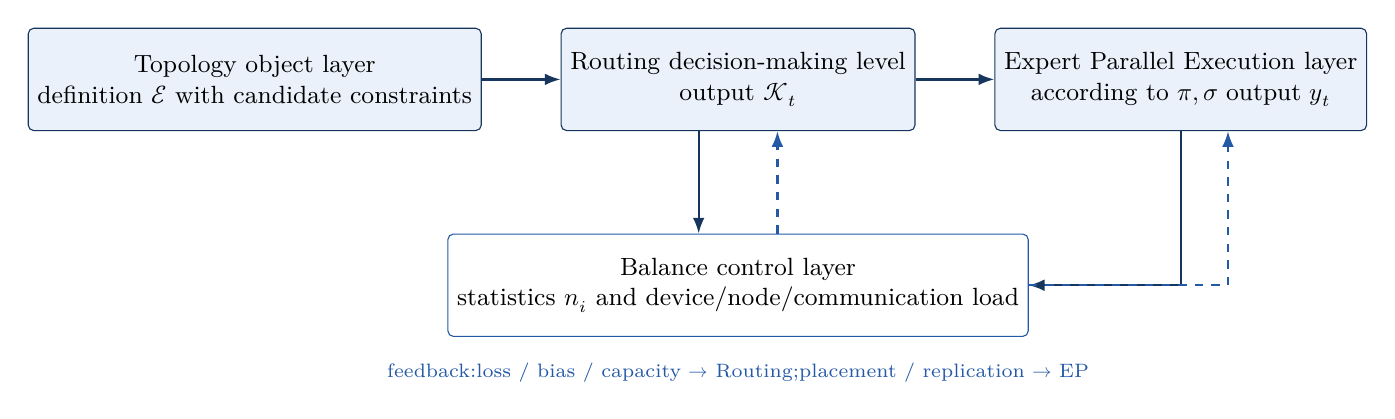
\begin{tikzpicture}[
  node distance=10mm and 10mm,
  plane/.style={draw=DeepBlue,rounded corners=2pt,fill=SoftBlue,minimum width=38mm,minimum height=13mm,align=center,font=\small},
  control/.style={draw=Accent,rounded corners=2pt,fill=white,minimum width=58mm,minimum height=13mm,align=center,font=\small},
  arr/.style={-{Latex[length=2mm]},thick,draw=DeepBlue},
  fb/.style={-{Latex[length=2mm]},thick,dashed,draw=Accent}
]
\node[plane] (topo) {Topology object layer\\definition $\mathcal{E}$ with candidate constraints};
\node[plane,right=of topo] (route) {Routing decision-making level\\output $\mathcal{K}_t$};
\node[plane,right=of route] (ep) {Expert Parallel Execution layer\\according to $\pi,\sigma$ output $y_t$};
\node[control,below=13mm of route] (bal) {Balance control layer\\statistics $n_i$ and device/node/communication load};
\draw[arr] (topo)--(route);
\draw[arr] (route)--(ep);
\draw[arr] ([xshift=-5mm]route.south)--([xshift=-5mm]bal.north);
\draw[fb] ([xshift=5mm]bal.north)--([xshift=5mm]route.south);
\draw[arr] (ep.south) |- (bal.east);
\draw[fb] (bal.east) -| ([xshift=6mm]ep.south);
\node[font=\scriptsize\color{Accent},below=2mm of bal] {feedback:loss / bias / capacity $\rightarrow$ Routing;placement / replication $\rightarrow$ EP};
\end{tikzpicture}
\caption{The closed-loop relationship between Topology, Routing, Balance and Expert Parallel. The first three solid lines form the forward execution chain, and the dashed lines represent the feedback of statistics and system costs on routing and placement.}
\label{fig:fourplanes}
\end{figure}

\begin{table}[htbp]
\centering
\caption{Criteria for the division of the four control planes}
\label{tab:fourplanes}
\small
\begin{tabularx}{\textwidth}{>{\raggedright\arraybackslash}p{0.17\textwidth}>{\raggedright\arraybackslash}p{0.22\textwidth}>{\raggedright\arraybackslash}p{0.25\textwidth}Y}
\toprule
Control plane & Core issue & Main status and time scale & Typical failure mode \\
\midrule
Topology object layer & What experts are there, how big are they and how are they grouped or shared & Weight structure; slow variables in architecture design/training period & Knowledge redundancy, too coarse granularity, too heavy sharing paths \\
Routing decision-making layer & Which experts should be selected for the current token, how many to activate & affinity, Top-$k$, candidate constraints; token-by-token fast variables & misrouting, discrete optimization is difficult, semantics are topologically constrained \\
Balance control layer & Whether the usage distribution of a set of tokens meets training and system goals & expert/device/node load; sequence to runtime multi-scale feedback & collapse, over-uniformity, straggler, communication hotspot \\
Expert Parallel execution layer & Where, with what communication pattern and kernels, the selected expert is executed & placement, dispatch/combine, scheduling; step/runtime variables & exposed All-to-All time, small GEMMs, P99 latency, GPU-memory hotspots \\
\bottomrule
\end{tabularx}
\end{table}

There are two types of reverse dependencies between the four layers that cannot be ignored. First, the physical topology will constrain semantic routing: in order to reduce fan-out, device-limited routing actively reduces the candidate set visible to a certain token in $\mathcal{E}$. Second, Balance does not just tune the Router: runtime replication or expert placement can improve the physical load without changing $\mathcal{K}_t$. Therefore, "load balancing" cannot only be understood as an auxiliary loss, and "Expert Parallel" is not a passive implementation that is intervened after the model structure is determined.

\section{Eight Evolutionary Milestones: Criteria, Mainline, and Branches}

The eight milestones are neither a fixed taxonomy copied from one survey nor a mechanical division by year. They are an analytical summary based on \term{migration of the dominant bottleneck}. A change qualifies as a milestone only if it satisfies three criteria. First, it introduces an independently adjustable design variable, such as Top-$k$, expert granularity, a shared path, or a dynamic active budget. Second, it moves the system's principal bottleneck, for example from compute growing linearly with the number of experts, to discrete routing and load imbalance, and then to All-to-All communication, small GEMMs, or weight I/O. Third, later architectures inherit the change, so it is more than a one-off implementation detail.

According to this standard, node 1--6 forms a clearer historical backbone: statistical division of labor $\rightarrow$ sparse activation $\rightarrow$ Transformer scale $\rightarrow$ decoder-only productization $\rightarrow$ fine-grained knowledge organization $\rightarrow$ ultra-sparse capacity expansion. Node 7 and node 8 are not simply new "generations" that follow node 6: Node 7 relaxes the assumption that "each token has a fixed amount of calculation"; node 8 relaxes the assumption that "semantic routing, intra-layer expert topology and physical communication must be bound". Both can be combined with the expert structure of node 5 or 6. Figure \ref{fig:evolution-dag} shows this inheritance relationship.

\begin{figure}[htbp]
\centering
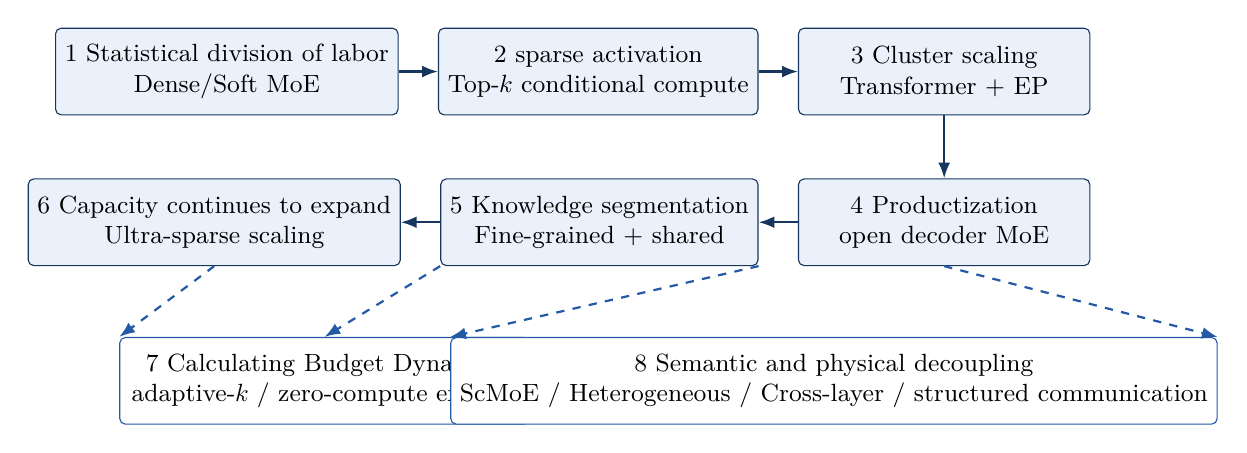
\begin{tikzpicture}[
  node distance=5mm and 5mm,
  stage/.style={draw=DeepBlue,rounded corners=2pt,fill=SoftBlue,minimum width=37mm,minimum height=11mm,align=center,font=\small},
  branch/.style={draw=Accent,rounded corners=2pt,fill=white,minimum width=52mm,minimum height=11mm,align=center,font=\small},
  arr/.style={-{Latex[length=2mm]},thick,draw=DeepBlue},
  darr/.style={-{Latex[length=2mm]},thick,dashed,draw=Accent}
]
\node[stage] (s1) {1 Statistical division of labor\\Dense/Soft MoE};
\node[stage,right=of s1] (s2) {2 sparse activation\\Top-$k$ conditional compute};
\node[stage,right=of s2] (s3) {3 Cluster scaling\\Transformer + EP};
\node[stage,below=8mm of s3] (s4) {4 Productization\\open decoder MoE};
\node[stage,left=of s4] (s5) {5 Knowledge segmentation\\Fine-grained + shared};
\node[stage,left=of s5] (s6) {6 Capacity continues to expand\\Ultra-sparse scaling};
\node[branch,below=9mm of s6,xshift=14mm] (s7) {7 Calculating Budget Dynamics\\adaptive-$k$ / zero-compute experts};
\node[branch,below=9mm of s4,xshift=-14mm] (s8) {8 Semantic and physical decoupling\\ScMoE / Heterogeneous / Cross-layer / structured communication};
\draw[arr] (s1)--(s2);
\draw[arr] (s2)--(s3);
\draw[arr] (s3)--(s4);
\draw[arr] (s4)--(s5);
\draw[arr] (s5)--(s6);
\draw[darr] (s5.south west)--(s7.north);
\draw[darr] (s6.south)--(s7.north west);
\draw[darr] (s5.south east)--(s8.north west);
\draw[darr] (s4.south)--(s8.north east);
\end{tikzpicture}
\caption{The relationship between eight evolution nodes. Solid lines represent primary inheritance on the historical trunk, and dashed lines represent stackable orthogonal branches; node numbers do not represent strict generational replacement.}
\label{fig:evolution-dag}
\end{figure}

\begin{table}[htbp]
\centering
\caption{Division basis of eight nodes and bottleneck migration}
\label{tab:evolution-nodes}
\small
\begin{tabularx}{\textwidth}{p{0.055\textwidth}p{0.18\textwidth}p{0.25\textwidth}Y}
\toprule
Node & New design variable & Dominant problem solved & New bottleneck transferred out \\
\midrule
1 & gating and expert specialization & It is difficult for a single model to model the input space partition & All experts calculate, and the capacity is bound to FLOPs \\
2 & sparse Top-$k$ and capacity & total parameters decoupled from active FLOPs & discrete routing, collapse, token drop \\
3 & EP, All-to-All, stabilization loss & Cluster-level training of Transformer MoE & Communication, straggler, numerical and load stability \\
4 & decoder-only training and deployment closed loop & proves that classic MoE can enter the open model ecosystem & big expert knowledge redundancy, coarse combination granularity \\
5 & fine-grained, shared, device limit & Public knowledge duplication and insufficient expert combination & fan-out, small GEMM, shared path fixed cost \\
6 & Larger $N$, tiny experts, retrieval routing & Continue to expand total capacity under fixed active budget & Weighted I/O, retrieval, low token/expert \\
7 & adaptive compute / zero slots & token has different difficulty but uses fixed Top-$k$ & active budget control, tail delay, training stability \\
8 & shortcut, heterogeneous/cross-layer topology, structured communication & Semantic routing is bound by device topology and communication & Scheduling complexity, cache consistency, large-scale verification \\
\bottomrule
\end{tabularx}
\end{table}

\subsection{Dense/Soft MoE: Statistical division of labor rather than computational sparsity}

Jacobs et al. proposed the basic form \cite{jacobs1991adaptive} of gating network and local experts in 1991. What this node establishes is \term{ statistical division of labor }: gate generates mixed weights according to the input, different sub-networks fit different areas of the input space, and the training goals can promote specialization. Since all experts usually participate in weighting, routing is continuously differentiable, requiring neither token capacity nor sparse dispatch in the All-to-All sense.

\textbf{Why is this a separate milestone?} It established three roles retained by later MoE systems: a router or gate, a set of experts, and a weighted combination operator. \textbf{Why is it not yet a modern sparse MoE?} Increasing the number of experts still increases compute approximately linearly, so model capacity and FLOPs per token remain coupled. The next milestone preserves statistical specialization while executing only a small subset of experts, enabling conditional scaling but introducing optimization and systems problems associated with discrete selection.

\subsection{Sparse conditional computation: Top-k establishes capacity leverage}

Shazeer et al. applied noisy Top-$k$ routing to very large sparse networks\cite{shazeer2017outrageously}, so that only a few experts execute for each input. If the total number of experts is $N$ and each input activates only $k\ll N$ experts, total capacity can grow with $N$ while the dominant expert FLOPs scale approximately with $k$. This establishes the central capacity lever of modern MoE: \term{parameter capacity is decoupled from per-token compute}.

This decoupling is not free. Top-$k$ causes unselected experts to have no gradient from this token; popular experts will overflow capacity, and unpopular experts may not be trained for a long time; dispatch/combine must also be added for cross-device execution. Therefore, noisy routing, importance/load auxiliary loss, capacity factor and token drop are not peripheral techniques, but supporting mechanisms induced by sparse execution itself. Node 3 does not change this basic algorithm, but answers: how to make MoE stable and executable when it is repeatedly embedded in Transformer layers and scaled to thousands of devices.

\subsection{Transformer MoE and Expert Parallel}

GShard systematically embeds Top-2 MoE FFN into Transformer and relies on automatic sharding to train \textbf{ on \textbf{2048 TPU} multi-language model \cite{lepikhin2020gshard} with more than 600B}. The classic execution chain is thus fixed as
\begin{center}
\textsf{Attention $\rightarrow$ Router $\rightarrow$ Dispatch All-to-All $\rightarrow$ Expert FFN $\rightarrow$ Combine All-to-All}.
\end{center}
The new variable of this node is not "more experts", but \term{expert parallelism and cluster execution semantics }: how tokens are rearranged across devices, how each expert is batch-processed, how overflows are handled, and how communication and calculation are synchronized. Switch Transformer further adopts Top-1, trading lower communication and simpler execution for expert combination capabilities and routing fault tolerance reduction \cite{fedus2021switch}. ST-MoE elevates stability to a first-class design goal and introduces Router z-loss constraint logits numerical scale \cite{zoph2022stmoe}. It needs to be distinguished: z-loss controls numerical stability, and balance loss controls usage distribution. The two are not the same mechanism.

During the same period, BASE Layers wrote the training route as a strictly balanced linear allocation problem \cite{lewis2021base}, while Expert Choice allowed experts to choose fixed capacity tokens \cite{zhou2022expertchoice}. They can directly guarantee equilibrium, but batch-level joint allocation and expert-side capacity are not as natural as token-choice for online autoregressive decoding, so they did not replace the Top-$k$ backbone of decoder-only LLM. The legacy of node 3 is the complete system contract of "Router + EP + capacity/balance + All-to-All"; nodes 4 and 5 both follow it, but shift the focus from "can large-scale training" to model quality, deployment availability and expert internal organization.

\subsection{Open-Weight Coarse-Grained MoE}

Mixtral uses \textbf{8$\times$7B parameters with Top-2 routing per token}\cite{jiang2024mixtral}. It did not introduce a new router family and therefore is not a milestone purely in terms of algorithmic novelty. Its importance is different: it demonstrated that \term{a conventional coarse-grained MoE can support pretraining, instruction tuning, inference deployment, and community reproduction} in an open-weight decoder-only LLM.

Why is this a \textbf{separate milestone}? Node 3 demonstrates scalable training on very large clusters; node 4 establishes an end-to-end path from pretraining and instruction tuning to practical deployment for a general-purpose decoder model. It inherits Top-$k$, isomorphic experts, and EP without changing the basic execution chain. Once the system can run reliably, the main bottleneck shifts to knowledge organization: a small number of large experts tend to relearn common capabilities, while the Router can compose only coarse knowledge blocks. Node 5 addresses this bottleneck directly.

\subsection{Shared + fine-grained experts}

DeepSeekMoE makes two key changes to coarse-grained experts\cite{dai2024deepseekmoe}. First, it splits a large FFN into multiple smaller experts, allowing the Router to compose more knowledge units under the same active budget. Second, shared-expert isolation moves knowledge needed by all tokens onto an always-on path, reducing redundancy among routed experts. The former increases \term{composition resolution}, while the latter explicitly separates common and conditional capabilities. DeepSeek-V2 scales this structure to \textbf{236B total parameters and 21B active parameters}, and adds device-limited routing: each token's candidate experts are restricted to a small number of devices, thereby controlling cross-device fan-out\cite{deepseekv2}.

Shared or dense paths can also provide computational windows that hide communications. DeepSeek-V2 combines shared expert computation with EP communication overlap; Snowflake Arctic's dense residual path also reflects the similar algorithm -- system collaboration \cite{snowflakearctic}. But \term{shared expert is not a necessary condition for fine-grained MoE }. Qwen3-235B-A22B uses \textbf{128 fine-grained experts and Top-8}, but removes the shared expert and relies on global-batch balance to allow commonly used capabilities to naturally form \cite{qwen3} among routed experts.

Therefore, node 5 actually contains two divisible axes: expert granularity and shared path. They are often combined, but there is no logical binding. Node 5 inherits the EP system of node 3, but increases the number of experts, Top-$k$, and device fan-out at the same time, making small GEMM, routing fragmentation, and communication topology new bottlenecks. Node 6 continues to expand along the lines of "more and smaller experts"; Node 8 attempts to change the physical implementation of fan-out and communication.

\subsection{Ultra-sparse scaling}

The question at this stage is: \emph{with active parameters fixed, does increasing the total number of experts continue to reduce loss?} PEER uses product-key retrieval to select a small subset from \textbf{more than one million tiny experts}\cite{he2024peer}. Kimi K2 scales an engineering-oriented ultra-sparse design to \textbf{1.04T total parameters, 32.6B active parameters, 384 routed experts, and Top-8 routing}, and reports scaling gains from higher sparsity at a fixed active budget\cite{kimiK2}. GPT-OSS-120B uses \textbf{128 experts with Top-4 routing} and a relatively small active footprint, illustrating an ultra-sparse design intended for local deployment\cite{openaiGptOss}.

\textbf{Why separate ultra-sparse scaling from fine-grained experts?} Fine-grained experts primarily reduce knowledge redundancy and increase composition resolution. Ultra-sparse scaling instead asks whether a larger candidate expert set continues to improve loss when active parameters and training FLOPs are fixed. Both increase expert count, but they optimize different objectives.

\term{Sparsity cannot increase without bound.} As $N$ grows, router scoring, expert-weight I/O, All-to-All metadata, and small-GEMM fragmentation all increase. When each expert receives too few tokens per step, \textbf{theoretical FLOP savings no longer translate into wall-clock gains}. Ultra-sparse scaling therefore depends more heavily on fine-grained organization and routing control rather than replacing them. The next two milestones relax different constraints of the fixed Top-$k$ mainline.

\subsection{Dynamic compute: from fixed Top-k to token-dependent budget}

Fixed Top-$k$ implies that every token receives the same number of expert FLOPs even when tokens differ in semantic difficulty and required capacity. LongCat-Flash introduces zero-computation experts: the router still selects a fixed number of slots, but some slots are identities, so actual FFN compute varies by token\cite{longcatFlash}. Adaptive-$k$, threshold routing, and zero-compute slots share the objective of \term{decoupling which experts are selected from how much computation is allocated}.

\textbf{Relationship to ultra-sparse scaling.} Ultra-sparse scaling expands the candidate capacity $N$ while usually keeping $k$ fixed; dynamic computation changes the actual $k_t$, or the effective FFN compute, for each token. The two approaches can be combined: the candidate pool remains large, while easy tokens receive less compute and difficult tokens receive more. The control objective consequently expands from expert load alone to the mean active budget, budget variance, per-expert load, and P99 latency. Constraining average training FLOPs does not guarantee tail latency because difficult tokens may cluster within a micro-batch or request window.

The remaining issue of dynamic computing is closed-loop control: if the Router determines both the semantic expert and the computing budget, the balance bias affects both specialization and throughput; if only the long-term average is constrained, short-term bursts may occur. Therefore, adaptive bias/PID feedback, budget loss and runtime admission control are supporting issues and cannot be solved by simply modifying Top-$k$.

\subsection{Semantic routing decoupled from physical execution}

Node 1--7 mainly changes Router's optional expert or active budget; node 8 changes the lower-level assumption: \term{ semantically selecting an expert does not mean that it must be executed immediately along the fixed intra-layer All-to-All path }. This node is not a single model family, but four frontier branches with a common goal.

\textbf{Execution-dependency rearrangement.} ScMoE does not change which experts a token selects; it changes the dependency graph. Its cross-layer shortcut lets routed experts consume an intermediate representation from the preceding layer while the current dense/shared path overlaps the dispatch/combine communication window\cite{cai2024scmoe}. It reduces exposed communication but does not directly solve routing skew. Figure~\ref{fig:scmoe} gives an abstract comparison.

\begin{figure}[htbp]
\centering
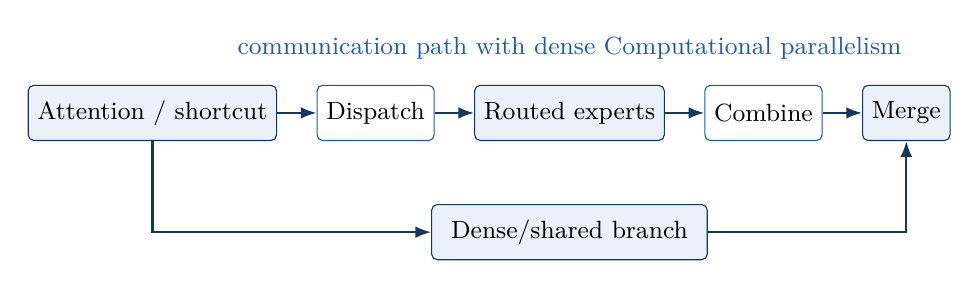
\begin{tikzpicture}[
  node distance=5mm and 5mm,
  box/.style={draw=DeepBlue,rounded corners=2pt,fill=SoftBlue,minimum height=7mm,align=center,font=\small},
  comm/.style={draw=Accent,rounded corners=2pt,fill=white,minimum height=7mm,align=center,font=\small},
  arr/.style={-{Latex[length=2mm]},thick,draw=DeepBlue}
]
\node[box] (attn) {Attention / shortcut};
\node[comm,right=of attn] (dispatch) {Dispatch};
\node[box,right=of dispatch] (expert) {Routed experts};
\node[comm,right=of expert] (combine) {Combine};
\node[box,right=of combine] (merge) {Merge};
\node[box,below=8mm of expert,minimum width=35mm] (dense) {Dense/shared branch};
\draw[arr] (attn)--(dispatch);
\draw[arr] (dispatch)--(expert);
\draw[arr] (expert)--(combine);
\draw[arr] (combine)--(merge);
\draw[arr] (attn.south) |- (dense.west);
\draw[arr] (dense.east) -| (merge.south);
\node[font=\small\color{Accent},above=2mm of expert] {communication path with dense Computational parallelism};
\end{tikzpicture}
\caption{At its core, ScMoE is about rearranging execution dependencies to expand the communication hidden window; it is not a new routing algorithm.}
\label{fig:scmoe}
\end{figure}

LongCat-Flash combines ScMoE with token-dimension chunking and Single Batch Overlap; the official LongCat-2.0 report further adopts fully parallel dense/MoE execution on each core of a dedicated accelerator\cite{longcat2}. These developments reduce exposed communication, \textbf{but they do not automatically eliminate severe routing skew, heterogeneous expert runtimes, or GPU-memory pressure}.

\textbf{Heterogeneous experts.} MoHGE uses two-level routing: it first selects an expert group and then experts of different sizes within that group, together with group-wise and intra-group balancing constraints\cite{mohge2026}. Equal expert width becomes a design variable rather than a default constraint, allowing different tokens to receive different forms of compute. The cost is greater complexity in heterogeneous GEMMs, capacity planning, and load metrics.

\textbf{Cross-layer sharing.} GMoE designates some experts as cross-layer Global Experts while retaining layer-local experts, reducing redundant capabilities across layers\cite{gmoe2026}. This differs from a conventional shared expert in scope: the former is reused across layers, whereas the latter is typically an always-on path within one layer. Cross-layer sharing introduces additional caching, scheduling, and inter-layer interference concerns.

\textbf{Structured communication.} Multi-Head LatentMoE and Head Parallel seek a topology whose communication volume is $O(1)$ with respect to the number of activated experts $k$, yielding more predictable traffic\cite{cui2026latentmoe}. Whereas ScMoE hides dynamic communication, this route attempts to reduce or structure the communication itself. In the absence of public validation at trillion-parameter and ten-thousand-accelerator scale, \term{it should be treated as a research frontier, not as a mainstream replacement for Top-$k$ expert parallelism}.

The four branches respectively optimize temporal overlap, computation structure, parameter reuse, and data movement. They are complementary and can be combined.

\section{Expert topology: object layer}

In the four-layer framework introduced in Chapter 2, Topology is the object layer. It defines the expert set $\mathcal{E}$, the granularity of each knowledge unit, the sharing scope, and computational heterogeneity before Routing makes token-level selections. The central question is therefore not simply how many experts exist, but \term{what kinds of computational units the router can compose}.

It is not sufficient to understand the evolution of MoE only as the growth of expert count. Table \ref{tab:topology} shows that what really changes is the granularity, sharing scope and computing heterogeneity of knowledge units.

\begin{table}[htbp]
\centering
\caption{The main evolution route of Expert topology}
\label{tab:topology}
\small
\begin{tabularx}{\textwidth}{p{0.21\textwidth}p{0.23\textwidth}Y Y}
\toprule
Topology & Representative work & Main benefit & New bottleneck \\
\midrule
A small number of isomorphic experts & GShard, Switch, Mixtral & Realize conditional scaling & Knowledge duplication, limited combinability \\
Shared/dense + routed & DeepSeekMoE, Arctic & Public knowledge isolation, can create overlap window & Fixed FLOPs increase, public path may be overweight \\
Fine-grained experts & DeepSeek-V2/V3, Qwen3 & Fine-grained experts combination, higher total/active ratio & Routing, communication and GEMM updated \\
Ultra-sparse experts & PEER, Kimi K2, gpt-oss & Continue to expand capacity under fixed FLOPs & Retrieval, weighted I/O, low token/expert \\
Heterogeneous/dynamic & LongCat, MoHGE & Token-level dynamic computing budget & budget control coupled with physical equalization \\
Cross-layer global/local & GMoE & Reduce cross-layer expert redundancy & Scheduling, caching and inter-layer interference need to be verified \\
Latent/head structured & Multi-Head LatentMoE & Communication deterministic, decoupled from $k$ & Insufficient evidence of large-scale quality \\
\bottomrule
\end{tabularx}
\end{table}

Another dimension that is often overlooked is the initialization method. Sparse Upcycling copies the existing dense FFN into multiple experts, and then adds a new Router to continue training \cite{komatsuzaki2022upcycling}. It reuses dense checkpoints, but brings expert symmetry. It requires routing noise, data differences and subsequent training to differentiate the experts. Further Expert Upcycling is extended from the existing $E$-expert MoE to $mE$ experts, while keeping Top-$k$ and active cost unchanged \cite{expertUpcycling2026}. Upcycling is not a new Router family, but it will change the formation path and training cost of specialization.

\section{Routing: decision-making layer}

In the closed loop of Figure~\ref{fig:fourplanes}, Routing receives the expert set defined by Topology and the candidate constraints imposed by the system, and generates $\mathcal{K}_t$ for each token. It optimizes \term{local semantic matching}; it does not directly guarantee a reasonable aggregate load over a sequence, batch, or device. The latter belongs to the Balance control plane discussed in Section~6.

\begin{table}[htbp]
\centering
\caption{Main Router families and their applicable boundaries}
\label{tab:router}
\small
\begin{tabularx}{\textwidth}{p{0.24\textwidth}p{0.19\textwidth}Y Y}
\toprule
Router family & Decision-making unit & Balance characteristics & decoder-only LLM Applicability \\
\midrule
Noisy Top-$k$ token-choice & token selection experts & requires loss, bias or runtime balance & current trunk, online naturally \\
Top-1 Switch & token choose 1 expert & Simple communication, more sensitive capacity & Expandable, but limited combination ability \\
Balanced assignment & batch joint assignment & Strictly equal during training & Global solution is complex and unnatural online \\
Expert-choice & expert select tokens & expert capacity is naturally fixed & encoder is more natural, decoder capacity is difficult to process \\
Soft/parameter merging & Continuous mixing & Differentiable, non-dispersion Top-$k$ & Large-scale EP efficiency not yet proven \\
Bias-controlled Top-$k$ & affinity + non-gradient bias & does not write the balanced gradient into the LM parameter & DeepSeek-V3 and other models use \\
Zero experts/adaptive-$k$ & token The amount of calculation is variable & The average budget and tail need to be constrained & The important direction of dynamic calculation \\
\bottomrule
\end{tabularx}
\end{table}

The fact that Token-choice has become mainstream does not mean that it is optimal in terms of optimization, but that it is the most consistent with the autoregressive online constraints: the routing of the current token only relies on the current state, and there is no need to wait for future tokens or solve the global distribution of the entire batch. Continuous routing schemes such as Soft MoE and Lory avoid discrete Top-$k$, but the system advantages have not yet been proven on ultra-large-scale decoder and low-latency EP\cite{puigcerver2023softmoe,zhong2024lory}.

Routing freedom is also constrained by network topology. Device-limited or node-limited routing limits candidate experts to a small number of devices/nodes to reduce single-token communication fan-out. The trade-off is that the semantically optimal expert may be excluded by topological constraints, so this type of design is inherently an explicit trade-off between quality and communication.

\section{Balance: control layer}

Balance does not redefine experts, nor does it independently generate semantic routes for tokens. It observes the $\{n_i\}$ and equipment, nodes and communication loads accumulated from many routing decisions, and then feeds back to the decision-making and execution layers through loss, bias, capacity or runtime placement. The core problem is: while \term{ allows uneven semantic specialization, how to avoid training collapse and physical straggler}.

\subsection{Sequence/batch-wise expert balance}

The classic auxiliary loss can be written as
\begin{equation}
  \mathcal{L}_{\mathrm{bal}}=\alpha N\sum_{i=1}^{N} f_i P_i,
  \label{eq:balance}
\end{equation}
Among them, $f_i$ is the token fraction actually assigned to expert $i$ in the statistical window, $P_i$ is the average routing probability, and $\alpha$ controls the equalization intensity. When all experts use approximately uniform values, the formula ~\eqref{eq:balance} is smaller. This loss is responsible for both preventing expert collapse and avoiding EP straggler, but they are not equivalent: the model may require uneven specialization, but the hardware hopes to have an even load. When $\alpha$ is too large, the hardware target directly interferes with the language modeling gradient.

\subsection{Device/node/communication-aware balance}

DeepSeek-V2 splits the balance into expert-level, device-level and communication balance, and controls fan-out\cite{deepseekv2} through device-limited routing. The key to this change is not to add a few more losses, but to acknowledge that \term{ logical expert balance is not equal to physical device or network balance }: If there are multiple experts on a device, as long as the total tokens between devices are close, it is not necessarily necessary that all experts are completely equal.

\subsection{Auxiliary-Loss-Free Load Balancing}

The Auxiliary-Loss-Free (ALF) strategy adds non-gradient routing bias $b_i$ to each expert:
\begin{equation}
  \mathcal{K}_t=\operatorname{TopK}_i(s_{i,t}+b_i),\qquad
  b_i\leftarrow b_i+\eta\,\operatorname{sign}(\bar n-n_i),
  \label{eq:alf}
\end{equation}
Where $\eta$ is the bias update speed. The bias affects the Top-$k$ selection, but does not participate in the LM gradient as an affinity weight, thereby reducing the direct interference of the equilibrium target on the model parameter update direction \cite{wang2024auxfree}. DeepSeek-V3 uses batch-wise ALF as the main balancing mechanism, while retaining a very weak sequence-wise auxiliary loss to prevent extreme single-sequence imbalance \cite{deepseekv3}. Therefore, \term{ "DeepSeek-V3 has no balance loss at all" is not accurate }.

Global-batch statistics are more stable than single micro-batch, and also allow some experts to carry more specific domain tokens on local batches; the cost is that load needs to be aggregated across DP/EP ranges, and expanding the statistical range may introduce additional communication.

\subsection{Runtime expert placement}

Balance on the training distribution cannot guarantee true inference traffic. Domain shift, SFT/RL and off balance updates all change expert popularity. DeepSeek-V3 uses redundant expert deployment, replicates hotspot experts and adjusts placement\cite{deepseekv3} at runtime. This trend re-partitions the goals: Routers can preserve semantically non-uniform specialization, and runtimes avoid device stragglers by copying, migrating, or relocating them.

\begin{figure}[htbp]
\centering
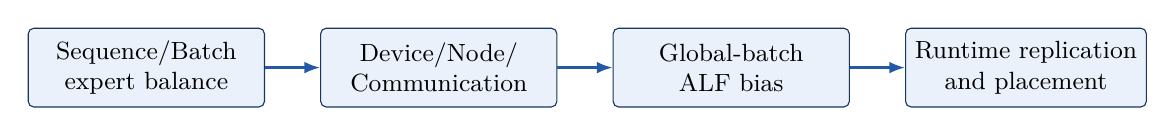
\begin{tikzpicture}[
  stage/.style={draw=DeepBlue,fill=SoftBlue,rounded corners=2pt,minimum width=30mm,minimum height=10mm,align=center,font=\small},
  arr/.style={-{Latex[length=2mm]},thick,draw=Accent}
]
\node[stage] (s1) {Sequence/Batch\\expert balance};
\node[stage,right=7mm of s1] (s2) {Device/Node/\\Communication};
\node[stage,right=7mm of s2] (s3) {Global-batch\\ALF bias};
\node[stage,right=7mm of s3] (s4) {Runtime replication\\and placement};
\draw[arr] (s1)--(s2);
\draw[arr] (s2)--(s3);
\draw[arr] (s3)--(s4);
\end{tikzpicture}
\caption{The evolution of Balance is not to simply weaken the constraints, but to gradually separate the physical execution goals from the LM gradient.}
\label{fig:balance}
\end{figure}

\section{Expert Parallel: Execution Layer}

EP consumes the token--expert assignment generated by Routing, and combines it with placement $\pi$ to convert the logical expert into dispatch, local GEMM and combine on the device. It usually does not change "who is semantically selected", but determines the wall-clock cost of this selection; when the system cost is too high, the first three layers will be reversely modified through device-limited routing, placement or architectural reconstruction.

The algorithmic benefits of MoE only hold true if the sparse execution is efficient. The capacity-based system reserves fixed token slots for each expert, and overflow tokens are discarded or used as residual, which can easily cause inconsistency between training and inference. MegaBlocks uses block-sparse kernels to implement dropless MoE, so that dynamic token shapes no longer require token dropping\cite{gale2022megablocks}. Systems such as Tutel dynamically select parallel and pipeline strategies to adapt to different cluster sizes.\cite{hwang2022tutel}.

As experts become thinner and Top-$k$ becomes larger, communication gradually becomes a first-class architectural constraint, driving three processing methods:
\begin{enumerate}
\item \term{ Limited communication topology }: device/node-limited routing reduces fan-out;
\item \term{ Hidden communication }: shared computation overlap, DualPipe, ScMoE and token chunking expand the overlap window;
\item \term{ Reconstruct communication }: Head Parallel and other solutions turn dynamic traffic into a more deterministic communication mode.
\end{enumerate}

Here \term{ must distinguish between "total All-to-All time" and "exposed communication time" }. If the communication is completely covered by the dense path, the marginal benefit of continuing to optimize the link bandwidth on the end-to-end step time will decrease; conversely, even if the total communication volume remains unchanged, as long as the critical path is shortened, the throughput may be significantly improved. Therefore, the training report should at least give the \textbf{ traffic volume, overlap ratio, exposed dispatch/combine, MFU and step-time P99}.

\section{The Modern Mainline and Frontier Branches}

As of 2026, the most common combinations of large-scale decoder MoE can be summarized as:
\begin{center}
\fcolorbox{DeepBlue}{SoftGray}{\parbox{0.88\textwidth}{\centering
Token-choice Top-$k$ + fine-grained experts + optional shared path + global/batch-wise balance or ALF + topology-limited routing + dropless kernels/communication overlap + runtime expert placement}}
\end{center}

DeepSeek-V3, Qwen3 and Kimi K2 differ in shared expert, balance mechanism and EP size, but they are all located on this backbone. At the same time, the following branches have not yet reached a unified conclusion:
\begin{itemize}
\item \term{MoE Attention}: JetMoE sparses Attention and FFN at the same time, further reducing active FLOPs, but KV/cache and routing are more complex \cite{shen2024jetmoe};
\item \term{Hybrid mixer + MoE}: Jamba alternates between Transformer and Mamba layers, indicating that MoE is a parameter expansion method and does not bind the full Attention backbone\cite{lieber2024jamba};
\item \term{Million experts}: High theoretical composability, but weighted I/O, small GEMM and retrieval overhead still limit industrial deployment;
\item \term{Heterogeneous experts}: Choose different capacities according to token difficulty, with natural expression, but physical placement and tail delay are more difficult;
\item \term{Cross-layer global experts}: The goal is to eliminate inter-layer duplication capabilities, but there is still a lack of evidence for very large-scale training;
\item \term{Structured communication}: Head Parallel may reduce the pain point of dynamic EP, but it is still in the early verification stage.
\end{itemize}

Table \ref{tab:models} compares representative models based on architecture selection rather than benchmark ranking.

\begin{table}[htbp]
\centering
\caption{Architectural location of representative LLM MoE; active parameter size varies by report}
\label{tab:models}
\scriptsize
\begin{tabularx}{\textwidth}{p{0.18\textwidth}C{15mm}C{25mm}C{22mm}Y}
\toprule
Model & Year & Total/Active & Experts/Top-$k$ & Architectural significance \\
\midrule
GShard & 2020 & $>$600B/Not uniformly disclosed & Top-2 & Transformer MoE with automatic sharding \\
Switch & 2021 & up to 1T+ & Top-1 & Exchange throughput and scalability with simple routing \\
Mixtral 8$\times$7B & 2024 & 46.7B/12.9B & 8/2 & Open coarse-grained MoE Benchmark \\
DeepSeek-V2 & 2024 & 236B/21B & 160/6 & fine-grained, shared, device-limited \\
DeepSeek-V3 & 2024 & 671B/37B & 256/8 & ALF, weak seq loss, node-limited \\
Qwen3-235B-A22B & 2025 & 235B/22B & 128/8 & fine-grained, no shared, global balance \\
Kimi K2 & 2025 & 1.04T/32.6B & 384/8 & ultra-sparse scaling \\
gpt-oss-120b & 2025 & 116.8B/5.1B & 128/4 & Small active footprint and deployment orientation \\
LongCat-Flash & 2025 & 560B/18.6--31.3B & real + zero & Dynamic Compute Budget with ScMoE \\
LongCat-2.0 & 2026 & 1.6T/33--56B & dynamic & dense/MoE per-core parallel \\
\bottomrule
\end{tabularx}
\end{table}

\section{Experimental Design for Foundation-Model Pretraining}

\term{ cross-model benchmark cannot identify architectural contributions. } To determine whether fine-grained, shared, ALF or ScMoE is effective, you should at least fix the \textbf{ training token, data ratio, active parameters and optimizer } at the same time, and report \textbf{training-FLOPs-matched and wall-clock-matched} result.

\begin{table}[htbp]
\centering
\caption{Proposed equal-budget MoE ablation matrix}
\label{tab:experiments}
\small
\begin{tabularx}{\textwidth}{p{0.20\textwidth}p{0.39\textwidth}Y}
\toprule
Experiment dimension & Recommendation setting & Core indicator \\
\midrule
Expert granularity & Fixed total/active params and tokens, scan expert count, width, Top-$k$ & val loss, downstream, token/expert, GEMM efficiency \\
Shared vs emergent & shared; no shared+global loss; no shared+ALF & expert similarity, domain-routing MI, active FLOPs \\
Balance scope & sequence aux, global aux, ALF, ALF+weak seq & max/mean load, CV/Gini, entropy, specialization \\
Execution topology & serial EP, shared overlap, ScMoE, runtime EPLB & exposed communication, MFU, step time, TPOT, P99 \\
Dynamic compute & fixed Top-$k$, threshold, zero experts & active-param mean/variance, bucketing loss, throughput and tail delay \\
Upcycling & scratch, dense-copy, cluster/utility-aware copy & Symmetry breaking speed, loss/token, GPU hours \\
\bottomrule
\end{tabularx}
\end{table}

For code pre-training scenarios, it is recommended to additionally bucket statistics by language, repo/file/function granularity, code and natural language token routing. Key observations include: expert co-activation in different languages, whether cross-file reference tokens are concentrated in a small number of experts, whether code and code-related documents share experts, and whether long repo-level sequences cause sequence-wise load peaks. Only in this way can we distinguish between "experts forming beneficial specialization" and "data matching causing accidental traffic skew".

The system side should at least record at the same time:
\begin{itemize}
\item max/mean, CV and Gini at the three levels of expert, device and node;
Load under the three statistical windows of \item sequence, micro-batch, and global batch;
\item dispatch/combine exposed time, not just the total All-to-All time;
  \item token drop, capacity overflow, redundant expert hit rate;
\item training FLOPs, active parameters, wall-clock and cluster network topology.
\end{itemize}

\section{Open Questions}

\subsection{What is the correct unit of analysis for Specialization?}

"Mathematical expert" or "code expert" are intuitive narratives, but actual routing is often represented by a combination of token morphology, syntax, location, language, and hierarchy. A single expert may not be a stable semantic unit, and a cross-layer expert group or co-activation pattern may be more interpretable. In the future, routing mutual information, expert representation similarity and intervention-based causal test should be combined instead of just showing token word cloud.

\subsection{Where Is the Systems Optimum at Higher Sparsity?}

Increasing total experts under fixed active FLOPs may reduce model loss, but system benefits are limited by network bandwidth, expert weight I/O, batch size and kernel arithmetic intensity. The optimal sparsity is not a pure model constant, but the model -- hardware joint scaling law. The EP size, network topology, and number of tokens per expert must be given when reporting this conclusion.

\subsection{Can Load Balancing Move Primarily to Runtime?}

ALF reduces the gradient interference of the auxiliary loss, but still changes the Top-$k$ selection. Runtime replication and placement can allow more freedom in semantic routing, but will bring parameter copy memory, migration costs and cache consistency issues. The optimal boundary between weak constraints in training and strong equilibrium at runtime remains undetermined.

\subsection{How Dynamic Compute Meets Tail Latency SLAs}

Zero experts or adaptive-$k$ can reduce average FLOPs, but difficult tokens will create new stragglers if they are in the same micro-batch or request window. The model needs to control average budget, budget variance, and P99 simultaneously, rather than just reporting average active parameters.

\subsection{How Can Post-Training Preserve Router Stability?}

SFT/RL data will change the domain distribution and sequence shape, thereby changing the expert load. Whether to retain balance updates, routing replay, and freeze Routers during the training phase cannot be directly extrapolated from the pre-training settings. Routing drift and specialization retention should be measured separately in the pretrain, SFT and RL stages.

\section{Summary and Outlook}

The architectural history of \term{LLM MoE is not a single-line expansion of "more and more experts", but the co-evolution of five routes: }expert has changed from a small number of large modules to fine-grained, ultra-sparse and heterogeneous computing units; the topology has developed from layer-local routed experts to shared, cross-layer global/local and latent-head structures; Router has evolved from simple Top-$k$ gradually adds global statistics, bias control and dynamic computing budget; balance moves from sequence-wise auxiliary loss to device/communication-aware, ALF and runtime placement; execution develops from serial All-to-All to dropless kernels, topology-limited routing, ScMoE overlap and structured communication.

Therefore, there is no unique "next-generation structure" after ScMoE. A more credible direction is a combination of four: freer semantic routing, explicit average computing budget control, topology awareness or deterministic communication, and runtime expert placement. Architecture evaluation must also be expanded from a single validation loss to a joint analysis of quality, specialization, active budget, exposed communication, and tail latency.

For the next round of large-scale pretraining, the most informative experiment is not a direct comparison of final benchmark scores from two different recipes. Instead, construct a controlled matrix with \textbf{the same data, token budget, and active FLOPs}, then vary expert granularity, the shared path, balancing scope, and execution topology separately. \textbf{This separation is necessary to distinguish gains from parameter capacity, routing specialization, and systems throughput}, and to derive MoE design conclusions that transfer to new hardware.

\appendix
\section{Architecture Evolution Cheat Sheet}

\begin{longtable}{@{}p{0.12\textwidth}p{0.19\textwidth}p{0.28\textwidth}p{0.30\textwidth}@{}}
\caption{Bottleneck migration of MoE architecture evolution}\label{tab:timeline}\\
\toprule
Period & Representative work & Main problems solved & New bottlenecks transferred out \\
\midrule
\endfirsthead
\toprule
Period & Representative work & Main problems solved & New bottlenecks transferred out \\
\midrule
\endhead
1991--2016 & Adaptive Mixtures & Learning soft division of labor & Computation increases linearly with the number of experts \\
2017--2019 & Sparse MoE & Parameter capacity and single token FLOPs decoupling & collapse, capacity, All-to-All \\
2020--2022 & GShard, Switch, ST-MoE & Transformer Large-scale sparse training & Stability, token drop, routing quality \\
2023--2024 & Mixtral & Open decoder MoE availability & Coarse-grained and knowledge redundant \\
2024--2025 & DeepSeekMoE/V2, Qwen3 & Fine-grained combination and public knowledge processing & Communication fan-out, small GEMM, balance scope \\
2024--2025 & PEER, Kimi K2, gpt-oss & ultra-sparse capacity expansion & retrieval, I/O, low token/expert \\
2024--2026 & ALF, LongCat, ScMoE & Reduce gradient interference and hidden communication & Runtime dynamic load and tail delay \\
2025--2026 & MoHGE, GMoE, Head Parallel & Heterogeneous computing, cross-layer sharing, structured communication & Ultra-large-scale quality and system verification \\
\bottomrule
\end{longtable}

\clearpage
\addcontentsline{toc}{section}{References}
\begin{thebibliography}{99}
\small
\setlength{\itemsep}{1pt}
\raggedright

\bibitem{cai2024survey}
Cai W, et al. A Survey on Mixture of Experts in Large Language Models. IEEE Transactions on Knowledge and Data Engineering, 2025. \url{https://arxiv.org/abs/2407.06204}.

\bibitem{liu2024inference}
Liu J, et al. A Survey on Inference Optimization Techniques for Mixture of Experts Models. arXiv:2412.14219, 2024. \url{https://arxiv.org/abs/2412.14219}.

\bibitem{zhu2025speed}
Zhu X, et al. Speed Always Wins: A Survey on Efficient Architectures for Large Language Models. arXiv:2508.09834, 2025. \url{https://arxiv.org/abs/2508.09834}.

\bibitem{jacobs1991adaptive}
Jacobs R A, Jordan M I, Nowlan S J, Hinton G E. Adaptive Mixtures of Local Experts. Neural Computation, 3(1):79--87, 1991. \href{https://doi.org/10.1162/neco.1991.3.1.79}{doi:10.1162/neco.1991.3.1.79}.

\bibitem{shazeer2017outrageously}
Shazeer N, et al. Outrageously Large Neural Networks: The Sparsely-Gated Mixture-of-Experts Layer. ICLR, 2017. \url{https://arxiv.org/abs/1701.06538}.

\bibitem{lepikhin2020gshard}
Lepikhin D, et al. GShard: Scaling Giant Models with Conditional Computation and Automatic Sharding. ICLR, 2021. \url{https://arxiv.org/abs/2006.16668}.

\bibitem{fedus2021switch}
Fedus W, Zoph B, Shazeer N. Switch Transformers: Scaling to Trillion Parameter Models with Simple and Efficient Sparsity. Journal of Machine Learning Research, 23(120):1--39, 2022. \url{https://arxiv.org/abs/2101.03961}.

\bibitem{zoph2022stmoe}
Zoph B, et al. ST-MoE: Designing Stable and Transferable Sparse Expert Models. arXiv:2202.08906, 2022. \url{https://arxiv.org/abs/2202.08906}.

\bibitem{lewis2021base}
Lewis M, et al. BASE Layers: Simplifying Training of Large, Sparse Models. ICML, 2021. \url{https://arxiv.org/abs/2103.16716}.

\bibitem{zhou2022expertchoice}
Zhou Y, et al. Mixture-of-Experts with Expert Choice Routing. NeurIPS, 2022. \url{https://arxiv.org/abs/2202.09368}.

\bibitem{jiang2024mixtral}
Jiang A Q, et al. Mixtral of Experts. arXiv:2401.04088, 2024. \url{https://arxiv.org/abs/2401.04088}.

\bibitem{dai2024deepseekmoe}
Dai D, et al. DeepSeekMoE: Towards Ultimate Expert Specialization in Mixture-of-Experts Language Models. ACL, 2024. \url{https://arxiv.org/abs/2401.06066}.

\bibitem{deepseekv2}
DeepSeek-AI. DeepSeek-V2: A Strong, Economical, and Efficient Mixture-of-Experts Language Model. arXiv:2405.04434, 2024. \url{https://arxiv.org/abs/2405.04434}.

\bibitem{snowflakearctic}
Snowflake. Arctic: Snowflake's Open-Source LLM. Official Technical Blog, 2024. Accessed 2026-08-07. \url{https://www.snowflake.com/en/blog/arctic-open-efficient-foundation-language-models-snowflake/}.

\bibitem{qwen3}
Qwen Team. Qwen3 Technical Report. arXiv:2505.09388, 2025. \url{https://arxiv.org/abs/2505.09388}.

\bibitem{he2024peer}
He X. Mixture of A Million Experts. arXiv:2407.04153, 2024. \url{https://arxiv.org/abs/2407.04153}.

\bibitem{kimiK2}
Moonshot AI. Kimi K2: Open Agentic Intelligence. arXiv:2507.20534, 2025. \url{https://arxiv.org/abs/2507.20534}.

\bibitem{openaiGptOss}
OpenAI. gpt-oss Model Card: Architecture. 2025. Accessed 2026-08-07. \url{https://deploymentsafety.openai.com/gpt-oss/architecture}.

\bibitem{longcatFlash}
LongCat Team. LongCat-Flash Technical Report. arXiv:2509.01322, 2025. \url{https://arxiv.org/abs/2509.01322}.

\bibitem{cai2024scmoe}
Cai W, et al. Shortcut-connected Expert Parallelism for Accelerating Mixture-of-Experts. arXiv:2404.05019, 2024. \url{https://arxiv.org/abs/2404.05019}.

\bibitem{longcat2}
LongCat Team. LongCat 2.0 Technical Blog. 2026. Accessed 2026-08-07. \url{https://longcat.ai/blog/longcat-2.0/}.

\bibitem{mohge2026}
MoHGE Authors. MoHGE: Mixture of Heterogeneous Grouped Experts. ACL Industry Track, 2026. \url{https://aclanthology.org/2026.acl-industry.20/}.

\bibitem{gmoe2026}
GMoE Authors. GMoE: Global Mixture-of-Experts. ACL, 2026. \url{https://aclanthology.org/2026.acl-long.2065/}.

\bibitem{cui2026latentmoe}
Cui Y, et al. Multi-Head LatentMoE and Head Parallel. arXiv:2602.04870, 2026. \url{https://arxiv.org/abs/2602.04870}.

\bibitem{komatsuzaki2022upcycling}
Komatsuzaki A, et al. Sparse Upcycling: Training Mixture-of-Experts from Dense Checkpoints. arXiv:2212.05055, 2022. \url{https://arxiv.org/abs/2212.05055}.

\bibitem{expertUpcycling2026}
Expert Upcycling Authors. Expert Upcycling: Training Larger MoE Models from Smaller MoE Checkpoints. arXiv:2604.19835, 2026. \url{https://arxiv.org/abs/2604.19835}.

\bibitem{puigcerver2023softmoe}
Puigcerver J, et al. From Sparse to Soft Mixtures of Experts. ICLR, 2024. \url{https://arxiv.org/abs/2308.00951}.

\bibitem{zhong2024lory}
Zhong Z, et al. Lory: Fully Differentiable Mixture-of-Experts for Autoregressive Language Model Pre-training. COLM, 2024. \url{https://arxiv.org/abs/2405.03133}.

\bibitem{wang2024auxfree}
Wang Q, et al. Auxiliary-Loss-Free Load Balancing Strategy for Mixture-of-Experts. arXiv:2408.15664, 2024. \url{https://arxiv.org/abs/2408.15664}.

\bibitem{deepseekv3}
DeepSeek-AI. DeepSeek-V3 Technical Report. arXiv:2412.19437, 2024. \url{https://arxiv.org/abs/2412.19437}.

\bibitem{gale2022megablocks}
Gale T, et al. MegaBlocks: Efficient Sparse Training with Mixture-of-Experts. MLSys, 2023. \url{https://arxiv.org/abs/2211.15841}.

\bibitem{hwang2022tutel}
Hwang C, et al. Tutel: Adaptive Mixture-of-Experts at Scale. MLSys, 2023. \url{https://arxiv.org/abs/2206.03382}.

\bibitem{shen2024jetmoe}
Shen Y, et al. JetMoE: Reaching Llama2 Performance with 0.1M Dollars. arXiv:2404.07413, 2024. \url{https://arxiv.org/abs/2404.07413}.

\bibitem{lieber2024jamba}
Lieber O, et al. Jamba: A Hybrid Transformer--Mamba Language Model. arXiv:2403.19887, 2024. \url{https://arxiv.org/abs/2403.19887}.

\end{thebibliography}

\end{document}
